%%%%%%%%%%%%%%%%%%%%%%%%%%%%%%%%%%%%%%%%%%%%%%%%

% Specify the command that you want into the header of the
% index.md file

%%%%%%%%%%%%%%%%%%%%%%%%%%%%%%%%%%%%%%%%%%%%%%%%

% Options for packages loaded elsewhere
\PassOptionsToPackage{unicode}{hyperref}
\PassOptionsToPackage{hyphens}{url}
\PassOptionsToPackage{dvipsnames,svgnames*,x11names*}{xcolor}
%
\documentclass[
  12pt,
  oneside]{report}
%%\usepackage{lmodern}
%
% Set line spacing
\usepackage{setspace}
\setstretch{1.5}

\usepackage{amssymb,amsmath}
\usepackage{ifxetex,ifluatex}
\ifnum 0\ifxetex 1\fi\ifluatex 1\fi=0 % if pdftex
  \usepackage[T1]{fontenc}
  \usepackage[utf8]{inputenc}
  \usepackage{textcomp} % provide euro and other symbols
\else % if luatex or xetex
  \usepackage{unicode-math}
  \defaultfontfeatures{Scale=MatchLowercase}
  \defaultfontfeatures[\rmfamily]{Ligatures=TeX,Scale=1}
\fi
% Use upquote if available, for straight quotes in verbatim environments
\IfFileExists{upquote.sty}{\usepackage{upquote}}{}
\IfFileExists{microtype.sty}{% use microtype if available
  \usepackage[]{microtype}
  \UseMicrotypeSet[protrusion]{basicmath} % disable protrusion for tt fonts
}{}
\makeatletter
\@ifundefined{KOMAClassName}{% if non-KOMA class
  \IfFileExists{parskip.sty}{%
    \usepackage{parskip}
  }{% else
    \setlength{\parindent}{0pt}
    \setlength{\parskip}{6pt plus 2pt minus 1pt}}
}{% if KOMA class
  \KOMAoptions{parskip=half}}
\makeatother
\usepackage{xcolor}
\IfFileExists{xurl.sty}{\usepackage{xurl}}{} % add URL line breaks if available
\IfFileExists{bookmark.sty}{\usepackage{bookmark}}{\usepackage{hyperref}}
\hypersetup{
  pdfauthor={François Leroy, PhD student at CZU},
  colorlinks=true,
  linkcolor=Blue,
  filecolor=Blue,
  citecolor=Blue,
  urlcolor=Blue,
  pdfcreator={LaTeX via pandoc}}
\urlstyle{same} % disable monospaced font for URLs

%% Package geometry
\usepackage[left = 2cm,right = 2cm,top = 2cm,bottom = 2cm]{geometry}
\usepackage{pdflscape}


%\usepackage{longtable} % out of date, now in latex-tools package
\usepackage{booktabs}
% Correct order of tables after \paragraph or \subparagraph
\usepackage{etoolbox}
\makeatletter
\patchcmd\longtable{\par}{\if@noskipsec\mbox{}\fi\par}{}{}
\makeatother
% Allow footnotes in longtable head/foot
\IfFileExists{footnotehyper.sty}{\usepackage{footnotehyper}}{\usepackage{footnote}}
\makesavenoteenv{longtable}
\usepackage{graphicx}
\makeatletter
\def\maxwidth{\ifdim\Gin@nat@width>\linewidth\linewidth\else\Gin@nat@width\fi}
\def\maxheight{\ifdim\Gin@nat@height>\textheight\textheight\else\Gin@nat@height\fi}
\makeatother
% Scale images if necessary, so that they will not overflow the page
% margins by default, and it is still possible to overwrite the defaults
% using explicit options in \includegraphics[width, height, ...]{}
\setkeys{Gin}{width=\maxwidth,height=\maxheight,keepaspectratio}
% Set default figure placement to htbp
\makeatletter
\def\fps@figure{htbp}
\makeatother
\setlength{\emergencystretch}{3em} % prevent overfull lines
\providecommand{\tightlist}{%
  \setlength{\itemsep}{0pt}\setlength{\parskip}{0pt}}
\setcounter{secnumdepth}{5}
%%% Complete the preamble of the LaTeX template
%%%------------------------------------------------------------------------------

%% Bug de bookdown: ne traite plus la déclaration "otherlangs" dans le préambule
% Pour charger les langues, écriture ici en dur du produit de bookdown
% Corrigé le 22/11/2019. A retester régulièrement: supprimer ces lignes si la compilation fonctionne sans elles.
\usepackage{polyglossia}
  \setmainlanguage[variant=american]{english}
  \setotherlanguage[]{french}
% Bug persistant le 28/02/2020

% Advised with polyglossia and babel
\usepackage{csquotes}

% Environnement "Essentiel" en début de chapitre
\usepackage[tikz]{bclogo}
\newenvironment{Essentiel}
  {\begin{bclogo}[logo=\bctrombone, noborder=true, couleur=lightgray!50]{L'essentiel}\parindent0pt}
  {\end{bclogo}}

%% Package fontspec
\usepackage{fontspec}
\setmainfont{calibri}[
  Path           = ./fonts/,
  Extension      = .ttf,
  BoldFont       = calibrib,
  ItalicFont     = calibrili,
  BoldItalicFont = calibriz]

% Rename chapters
% Below, scrpit to prevent the "chapter n" and the space use for it to
% be displayed
\usepackage{titlesec}
\titleformat{\chapter}   
{\Huge}{\thechapter{. }}{0pt}{\Huge}
%{\thechapter{. }}
\titlespacing*{\chapter}{0pt}{0pt}{10pt}
% empty space is to up the title and 10 is the space with the text below


% When using the natbib biblio package, includes "References" in the table of contents
\usepackage[nottoc]{tocbibind}

% To make the table caption full page width
\usepackage{caption}

% Make the figure float
\usepackage{float}

% In order to make the new chapter to start on the same page
\titleclass{\chapter}{straight}
\usepackage{float}
\usepackage{booktabs}
\usepackage{longtable}
\usepackage{array}
\usepackage{multirow}
\usepackage{wrapfig}
\usepackage{colortbl}
\usepackage{pdflscape}
\usepackage{tabu}
\usepackage{threeparttable}
\usepackage{threeparttablex}
\usepackage[normalem]{ulem}
\usepackage{makecell}
\usepackage{xcolor}
\ifluatex
  \usepackage{selnolig}  % disable illegal ligatures
\fi
\usepackage[style=apa,]{biblatex}
\addbibresource{references.bib}

\author{François Leroy, PhD student at CZU}
\date{2021-09-30}

% to include pdf
\usepackage{pdfpages}



%%%%%%%%%%%%%%%%%%%%%%%%%%%%%%%%%%%%%%%%%%%%%%%%%%%%%%%%%%%%%
% Start of the documents
\begin{document}

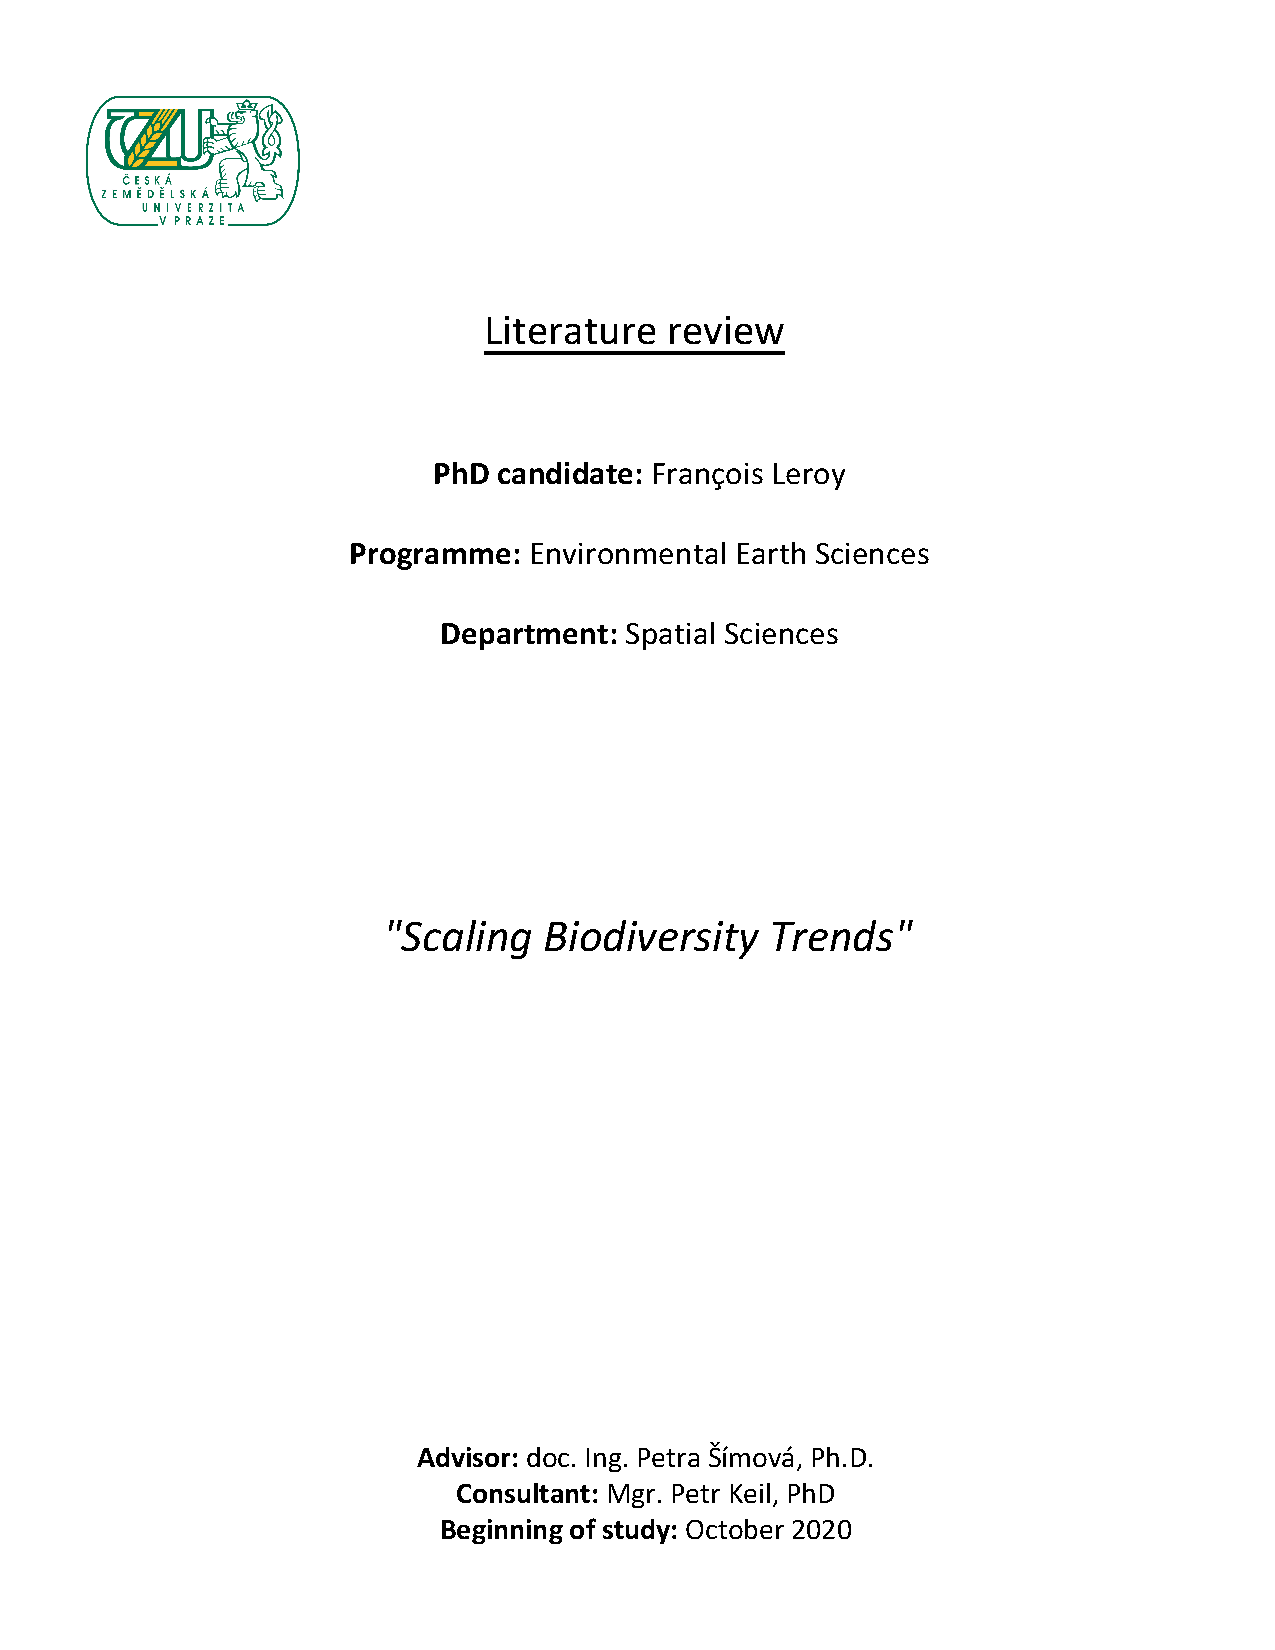
\includepdf[pages = {1}, fitpaper=true]{_assets/coverpage.pdf}

% Roman numbering for content before toc and toc itself
\cleardoublepage 
\pagenumbering{roman}

{
\hypersetup{linkcolor=}
\setcounter{tocdepth}{1}
\tableofcontents
\newpage
}
\vspace{50mm}
\setstretch{1.5}


% Start the arabic numbering at the 1st chapter
\cleardoublepage 
\pagenumbering{arabic}


% The mind, the...
\hypertarget{introduction}{%
\chapter{Introduction}\label{introduction}}

Our life quality is intrinsically linked to the state of ecosystems that we live in. Ecosystem services to humans \autocite{diaz_assessing_2018}, as well as their inner functioning, involve a spectrum of mechanisms including nutrient cycles or ecosystem stability \autocite{pereira_global_2012}. Some of these functions, such as seed dispersal, control of pests, scavenging, or pollination, depend on birds and their diversity. Birds also have a significant esthetical value, with most countries having numerous iconic/charismatic species of conservation interest (\url{https://www.iucnredlist.org/}). Moreover, given their ability to quickly move between locations, their presence is also a good indicator for ecosystem health. Unfortunately, anthropogenic stressors like habitat loss, over-exploitation, pollution, or introduction of invasive species are a threat to birds and their biodiversity \autocite{donald_agricultural_2001,jiguet_population_2010}, with concerns that they could face a sixth mass extinction \autocite{barnosky_has_2011}.

We have reasons to suspect that the global alteration of biodiversity due to anthropogenic stressors is unprecedented, and political goals have been declared in order to limit it \autocite[\emph{e.g.}][]{secretariat_of_the_convention_on_biological_diversity_global_2006}. However, data-driven basis for these policies remains a challenge, mainly due to severe gaps and biases in empirical biodiversity data \autocite{meyer_global_2015}. To complicate matters further, current scientific literature has shown that temporal trends of local biodiversity can be opposite to trends at larger spatial scales \autocites[\emph{e.g.}][]{chase_species_2019,keil_biodiversity_2011,keil_spatial_2018}. Thus, we should expect changes in biodiversity to be far more complex than a simple global decrease. Finally, biodiversity can be measured by many metrics, and these can differ in their temporal trends \autocite{mcgill_fifteen_2015}: for instance, while there may be small average net change in local species richness, ecosystems can still undergo significant changes in species composition \autocite{blowes_geography_2019,dornelas_quantifying_2013,vaidyanathan_worlds_2021}.

Particularly the issue of scale is critical \autocite{levin_problem_1992}. Since \textcite{arrhenius_species_1921} and \textcite{grinnell_role_1922}, we know that spatial and temporal scaling of biodiversity affects macroecological patterns. Even though particularly the static spatial scaling of biodiversity has been of great interest \autocite[\emph{e.g.}][]{storch_scaling_2007}, wonders persist about how temporal trends of biodiversity are linked to the spatial and temporal scales. In other words: does the observed biodiversity trends differ if we zoom out from local communities to regions, countries or continents? Here, the term ``spatial grain'' is also used to refer to the spatial scale of biodiversity, \emph{i.e.} the area at which the metric of biodiversity is assessed. One should be careful to not confuse spatial grain with the spatial extent of a study, \emph{i.e.} the total area of the ecosystem which is observed or analyzed \autocite{dungan_balanced_2002}. The same terminology is applied for the temporal scale: temporal grain refers to the temporal unit of the measured biodiversity \autocite{adler_power_2003}. Compared to spatial scaling, the temporal scaling is much less studied, which is mostly due to the lack of temporally replicated data. This review will, in part, show how the definition of temporal grain has still no consensus in the scientific literature.

To investigate the link between spatio-temporal grains and trends of biodiversity, birds are a relevant taxon. Thanks to the many ornithological monitoring initiatives and surveys, we have a large number of high-quality time series on bird populations \autocites{bejcek_velke_2016,kamp_population_2021,sauer_north_2013}. This is because birds are easy to observe, easy to identify and thus many volunteers are motivated to participate on citizen-science projects \autocite[\url{https://www.inaturalist.org/}]{sullivan_ebird_2009} or to conduct standardized sampling (\emph{e.g.} most of the breeding bird surveys are conducted by volunteers).

Given birds importance to assess ecosystem health, several standardized metrics have been created to assess their populations. \textcite{fraixedas_state_2020} reviewed this wide spectrum of bird biodiversity indicators, without considerations to their link with spatial and temporal grains. Here, we review articles assessing the temporal trends of avian biodiversity, with species focus on the variety of metrics that they use, and spatial and temporal scales at which temporal trends have been assessed. We consider the most common macroecological indicators used to assess biodiversity at the community level and higher, such as diversity indexes (\emph{e.g.} species richness, functional diversity) or population indexes \autocite{mcgill_fifteen_2015}. We highlight a lack of consensus about specifications and definitions of both spatial and temporal grains (respectively) of trends, we demonstrate that the scaling of trends is seldom considered, leading to confused messages about overall trends. Moreover, we show that studies lack spatial replication that would make reported trends robust and general. We believe that this review will improve the current knowledge on spatio-temporal scaling of trends biodiversity, and thus be useful for the ornithological field community and the conservation decision making.

\hypertarget{metrics-and-indicators}{%
\chapter{Metrics and indicators}\label{metrics-and-indicators}}

Studying biodiversity can be confusing as it exists many ways to measure it. The different metrics and indicators have diverse features, and one should consider which one is the most suited to its study. First, the type of biodiversity studied must be chosen (\emph{e.g.} taxonomic, functional, phylogenetic diversity). Only then, one must choose the metric(s).

\textbf{Classical metrics.} Measures of static biodiversity are commonly used such as local species richness (\(\alpha\) diversity), regional richness \autocite[\(\gamma\) diversity,][]{whittaker_vegetation_1960}, by indices that consider abundances \autocites[\emph{e.g.}][]{shannon_mathematical_1948,simpson_measurement_1949}, or by Hill numbers \autocite{hill_diversity_1973}. On the other hand, change of species composition in space and time can be expressed as \(\beta = \frac{\gamma}{\alpha}\) \autocite{whittaker_evolution_1972}, or by pairwise dissimilarity among locations or time periods \autocite{koleff_measuring_2003}. All these metrics assess species-based metrics, \emph{i.e.} they use the species as a unit. However, it has also been shown that functional and phylogenetic diversity can provide supplementary information on the community structure and its dynamic \autocites[\emph{e.g.}][]{mcgill_rebuilding_2006,mouquet_ecophylogenetics_2012,webb_phylogenies_2002}.

\textbf{Composite and multi-species indicators.} The composite indicators are made to summarize several ecosystem information into one informative index. The most known ones are the Red List Index \autocite{butchart_improvements_2007,butchart_measuring_2004,butchart_using_2005}, the Living Planet Index \autocite{loh_living_2005} or the Biodiversity Change Index \autocite{normander_indicator_2012}. In these composite indicators, metrics of great interest are the abundance-based or population-based metrics. As individuals react to stress or disturbances, the population trends reflect ecosystems health. The population decline that a species undergoes before going locally extinct is not captured by species-based metrics. Thus, population trends are usually efficient at assessing finer biodiversity declines. Although overall abundance is often hard to assess, the abundance of few indicator species can reflect processes in an entire ecosystem \autocite{gregory_developing_2005}. This has led to a proposition of a family of metrics called the multi-species indicators \autocite[MSI,][]{landres_ecological_1988}. Examples are the farmland bird indicator, woodland bird indicator or Wildland Bird Indicator which summarizes the latter two \autocite{gregory_generation_1999,gregory_wild_2010}. These metrics compute the geometric mean of abundance of few key species over time.

\hypertarget{quantitative-literature-review}{%
\chapter{Quantitative literature review}\label{quantitative-literature-review}}

For this review, we focused on articles assessing temporal trends of the most common metrics of avian biodiversity and specifying spatial and temporal scales, which are at the same time consistent with broader macroecological scaling and theory \autocite{storch_scaling_2007,storch_untangling_2004}, and thus can be compared across studies and scales. Namely, these were: \emph{Species richness, Evenness, Abundance, Diversity, Temporal beta-diversity, Spatial beta-diversity, Functional diversity, Functional evenness, Functional richness}. Some of these classes contain several different indexes. For instance, the class \emph{Diversity}, which contains either the Shannon or Simpson index, or the class \emph{Abundance}, which contains various multi-species indicators (see Table \ref{tab:notetable} for the notes).

We only considered articles for which there were spatial replicates, \emph{i.e.} where the trend of the metric was assessed at several locations at a given spatial grain. With these replications, the trend reported at one spatial grain is more reliable and general. However, at larger spatial grains (\emph{i.e.} national, continental or global scales), spatial replicates are rare. Thus, we considered these trends from a single location only when based on a large set of observations from smaller spatial scales.

We used the ``advanced search'' tool of the ISI Web of Science Core collection database with these four following queries:

\begin{enumerate}
\def\labelenumi{\arabic{enumi}.}
\item
  \texttt{AB\ =\ ((biodiversity\ OR\ species\ richness\ OR\ diversity)\ AND\ (temporal\ trend*\ OR\ dynamic*)\ AND\ (bird*\ OR\ avia*))} which resulted in 1346 references.
\item
  \texttt{AB\ =\ ((biodiversity\ change\ index)\ \ AND\ (bird*\ \ OR\ avia*)\ \ AND\ trend*)} which resulted in 60 references.
\item
  \texttt{AB\ =\ ((species\ richness)\ AND\ (bird*\ OR\ avia*)\ AND\ trend*)} which resulted in 313 references.
\item
  \texttt{ALL=(birds\ AND\ species\ richness\ AND\ temporal\ trend)} which resulted in 88 references.
\end{enumerate}

For each query, the title and abstract of these articles were reviewed. In addition, we scanned the references of these articles for other potentially relevant literature. When the temporal trend was explicitly reported (either in a graph or text), we extracted from the material and methods the type of metric, the spatial grain of the trend (\emph{i.e.} the area at which the metric trend is assessed), its temporal grain, the spatial extent (\emph{i.e.} the entire area on which the study applies), the temporal extent and the beginning and ending years of the study as well as the general trend of the metric (Table \ref{tab:maintable}). We discretized spatial grain sizes discretized into four levels: local \(<=25\) \(Km^2\), regional \(>25\) \(Km²\), national when an entire country was considered, and global at the worldwide scale (grain = extent = the entire Earth's mainland).

Concerning the trend assessment, different papers contain the \(p-value\) or directly specify the significance of a trend of a metric. However, some papers give only graphical representations of the trend. For those, the standard error was used when displayed. If a study only gave the trend, this is noted in the column \emph{Note} of the Table \ref{tab:notetable}. Moreover, the final trend retained (\emph{i.e.} either \emph{Increase}, \emph{Stable} or \emph{Decrease}) doesn't reflect all the fluctuations of the metric through time but rather the difference between the starting and ending points.

We found 31 references in which authors were both determining the temporal trend of a metric and explicitly defining the grain size. However, only 17 of them used spatial replicates and were thus relevant for this study (Table \ref{tab:maintable}).

\begin{landscape}\begingroup\fontsize{10}{12}\selectfont

\begin{longtable}[t]{>{\raggedright\arraybackslash}p{6.5em}>{\raggedright\arraybackslash}p{6.5em}>{\raggedright\arraybackslash}p{6.5em}>{\raggedleft\arraybackslash}p{6.5em}>{\raggedleft\arraybackslash}p{6.5em}>{\raggedleft\arraybackslash}p{6.5em}>{\raggedright\arraybackslash}p{6.5em}>{\raggedright\arraybackslash}p{6.5em}>{\raggedright\arraybackslash}p{6.5em}}
\caption{\label{tab:maintable}Trends of different metrics of biodiversity at various spatial and temporal scales}\\
\toprule
Reference & Metric & Spatial grain (Km²) & Temporal grain (year) & Spatial extent (Km²) & Temporal extent (year) & Years & Country & Trend\\
\midrule
\endfirsthead
\caption[]{\label{tab:maintable}Trends of different metrics of biodiversity at various spatial and temporal scales \textit{(continued)}}\\
\toprule
Reference & Metric & Spatial grain (Km²) & Temporal grain (year) & Spatial extent (Km²) & Temporal extent (year) & Years & Country & Trend\\
\midrule
\endhead

\endfoot
\bottomrule
\endlastfoot
\cellcolor{gray!6}{\cite{barnagaud_temporal_2017}} & \cellcolor{gray!6}{Evenness} & \cellcolor{gray!6}{Local} & \cellcolor{gray!6}{1.0} & \cellcolor{gray!6}{9834000} & \cellcolor{gray!6}{41} & \cellcolor{gray!6}{1970-2011} & \cellcolor{gray!6}{USA} & \cellcolor{gray!6}{Increase}\\
 & SR & Local & 1.0 & 9834000 & 41 & 1970-2011 & USA & Increase\\
\cellcolor{gray!6}{\cite{bowler_geographic_2021}} & \cellcolor{gray!6}{Abundance} & \cellcolor{gray!6}{National} & \cellcolor{gray!6}{1.0} & \cellcolor{gray!6}{520475} & \cellcolor{gray!6}{27} & \cellcolor{gray!6}{1990-2016} & \cellcolor{gray!6}{Czech Rep., Switzerland, Denmark, Germany} & \cellcolor{gray!6}{Stable}\\
\cite{chase_species_2019} & SR & Local & 5.0 & 2800000 & 30 & 1982–2011 & USA, Canada & Stable\\
\cellcolor{gray!6}{} & \cellcolor{gray!6}{SR} & \cellcolor{gray!6}{Regional} & \cellcolor{gray!6}{5.0} & \cellcolor{gray!6}{2800000} & \cellcolor{gray!6}{30} & \cellcolor{gray!6}{1982–2011} & \cellcolor{gray!6}{USA, Canada} & \cellcolor{gray!6}{\vphantom{1} Stable}\\
\addlinespace
 & SR & Regional & 5.0 & 2800000 & 30 & 1982–2011 & USA, Canada & Stable\\
\cellcolor{gray!6}{} & \cellcolor{gray!6}{SR} & \cellcolor{gray!6}{Local} & \cellcolor{gray!6}{5.0} & \cellcolor{gray!6}{2800000} & \cellcolor{gray!6}{30} & \cellcolor{gray!6}{1982–2011} & \cellcolor{gray!6}{USA, Canada} & \cellcolor{gray!6}{\vphantom{1} Increase}\\
 & SR & Local & 5.0 & 2800000 & 30 & 1982–2011 & USA, Canada & Increase\\
\cite{chiron_forecasting_2013} & Abundance & Regional & 1.0 & 643801 & 14 & 2007-2020 & France & \vphantom{2} Decrease\\
\cellcolor{gray!6}{} & \cellcolor{gray!6}{Abundance} & \cellcolor{gray!6}{Regional} & \cellcolor{gray!6}{1.0} & \cellcolor{gray!6}{643801} & \cellcolor{gray!6}{14} & \cellcolor{gray!6}{2007-2020} & \cellcolor{gray!6}{France} & \cellcolor{gray!6}{\vphantom{1} Decrease}\\
\addlinespace
 & Abundance & Regional & 1.0 & 643801 & 14 & 2007-2020 & France & Decrease\\
 & Abundance & Regional & 1.0 & 643801 & 14 & 2007-2020 & France & Decrease\\
\cellcolor{gray!6}{\cite{davey_rise_2012}} & \cellcolor{gray!6}{Diversity} & \cellcolor{gray!6}{Local} & \cellcolor{gray!6}{1.0} & \cellcolor{gray!6}{242495} & \cellcolor{gray!6}{13} & \cellcolor{gray!6}{1994-2006} & \cellcolor{gray!6}{UK} & \cellcolor{gray!6}{Increase}\\
 & Evenness & Local & 1.0 & 242495 & 13 & 1994-2006 & UK & Increase\\
\cellcolor{gray!6}{} & \cellcolor{gray!6}{SR} & \cellcolor{gray!6}{Local} & \cellcolor{gray!6}{1.0} & \cellcolor{gray!6}{242495} & \cellcolor{gray!6}{13} & \cellcolor{gray!6}{1994-2006} & \cellcolor{gray!6}{UK} & \cellcolor{gray!6}{Increase}\\
\addlinespace
\cite{harrison_assessing_2014} & Abundance & Local & 1.0 & 200000 & 18 & 1994-2011 & Great Britain, UK & Increase\\
\cellcolor{gray!6}{} & \cellcolor{gray!6}{Abundance} & \cellcolor{gray!6}{Local} & \cellcolor{gray!6}{1.0} & \cellcolor{gray!6}{200000} & \cellcolor{gray!6}{18} & \cellcolor{gray!6}{1994-2011} & \cellcolor{gray!6}{Great Britain, UK} & \cellcolor{gray!6}{\vphantom{1} Stable}\\
 & Abundance & Local & 1.0 & 200000 & 18 & 1994-2011 & Great Britain, UK & Stable\\
\cellcolor{gray!6}{\cite{harrison_quantifying_2016}} & \cellcolor{gray!6}{Abundance} & \cellcolor{gray!6}{Local} & \cellcolor{gray!6}{0.5} & \cellcolor{gray!6}{242495} & \cellcolor{gray!6}{20} & \cellcolor{gray!6}{1994-2013} & \cellcolor{gray!6}{UK} & \cellcolor{gray!6}{Increase}\\
 & Abundance & Local & 0.5 & 242495 & 20 & 1994-2013 & UK & \vphantom{1} Stable\\
\addlinespace
\cellcolor{gray!6}{} & \cellcolor{gray!6}{Abundance} & \cellcolor{gray!6}{Local} & \cellcolor{gray!6}{0.5} & \cellcolor{gray!6}{242495} & \cellcolor{gray!6}{20} & \cellcolor{gray!6}{1994-2013} & \cellcolor{gray!6}{UK} & \cellcolor{gray!6}{Stable}\\
\cite{jarzyna_taxonomic_2018}\cellcolor{gray!6}{} & \cellcolor{gray!6}{SR} & \cellcolor{gray!6}{Regional} & \cellcolor{gray!6}{1.0} & \cellcolor{gray!6}{9834000} & \cellcolor{gray!6}{45} & \cellcolor{gray!6}{1969-2013} & \cellcolor{gray!6}{USA} & \cellcolor{gray!6}{\vphantom{1} Increase}\\
 & SR & Regional & 1.0 & 9834000 & 45 & 1969-2013 & USA & Increase\\
 & SR & Regional & 1.0 & 9834000 & 45 & 1969-2013 & USA & Increase\\
\cellcolor{gray!6}{} & \cellcolor{gray!6}{SR} & \cellcolor{gray!6}{National} & \cellcolor{gray!6}{1.0} & \cellcolor{gray!6}{9834000} & \cellcolor{gray!6}{45} & \cellcolor{gray!6}{1969-2013} & \cellcolor{gray!6}{USA} & \cellcolor{gray!6}{Increase}\\
\addlinespace
 & SR & Global & 1.0 & 148940000 & 45 & 1969-2013 & World & Decrease\\
\cellcolor{gray!6}{} & \cellcolor{gray!6}{Temporal beta-diversity} & \cellcolor{gray!6}{Regional} & \cellcolor{gray!6}{1.0} & \cellcolor{gray!6}{9834000} & \cellcolor{gray!6}{45} & \cellcolor{gray!6}{1969-2013} & \cellcolor{gray!6}{USA} & \cellcolor{gray!6}{\vphantom{2} Increase}\\
 & Temporal beta-diversity & Regional & 1.0 & 9834000 & 45 & 1969-2013 & USA & \vphantom{1} Increase\\
\cellcolor{gray!6}{} & \cellcolor{gray!6}{Temporal beta-diversity} & \cellcolor{gray!6}{Regional} & \cellcolor{gray!6}{1.0} & \cellcolor{gray!6}{9834000} & \cellcolor{gray!6}{45} & \cellcolor{gray!6}{1969-2013} & \cellcolor{gray!6}{USA} & \cellcolor{gray!6}{Increase}\\
 & Temporal beta-diversity & National & 1.0 & 9834000 & 45 & 1969-2013 & USA & Increase\\
\addlinespace
\cellcolor{gray!6}{} & \cellcolor{gray!6}{Temporal beta-diversity} & \cellcolor{gray!6}{Global} & \cellcolor{gray!6}{1.0} & \cellcolor{gray!6}{148940000} & \cellcolor{gray!6}{45} & \cellcolor{gray!6}{1969-2013} & \cellcolor{gray!6}{World} & \cellcolor{gray!6}{Stable}\\
\cite{pilotto_meta-analysis_2020} & Abundance & Local & NA & 10180000 & NA & NA & Europe & Stable\\
\cellcolor{gray!6}{} & \cellcolor{gray!6}{Diversity} & \cellcolor{gray!6}{Local} & \cellcolor{gray!6}{NA} & \cellcolor{gray!6}{10180000} & \cellcolor{gray!6}{NA} & \cellcolor{gray!6}{NA} & \cellcolor{gray!6}{Europe} & \cellcolor{gray!6}{Increase}\\
 & SR & Local & NA & 10180000 & NA & NA & Europe & Increase\\
\cellcolor{gray!6}{} & \cellcolor{gray!6}{Temporal beta-diversity} & \cellcolor{gray!6}{Local} & \cellcolor{gray!6}{NA} & \cellcolor{gray!6}{10180000} & \cellcolor{gray!6}{NA} & \cellcolor{gray!6}{NA} & \cellcolor{gray!6}{Europe} & \cellcolor{gray!6}{Stable}\\
\addlinespace
\cite{ram_what_2017} & Abundance & Local & 1.0 & 350000 & 18 & 1998-2015 & Sweden & Increase\\
\cellcolor{gray!6}{} & \cellcolor{gray!6}{SR} & \cellcolor{gray!6}{Regional} & \cellcolor{gray!6}{1.0} & \cellcolor{gray!6}{350000} & \cellcolor{gray!6}{18} & \cellcolor{gray!6}{1998-2015} & \cellcolor{gray!6}{Sweden} & \cellcolor{gray!6}{Increase}\\
\cite{reif_changes_2013} & Spatial beta-diversity & Local & 1.0 & 79000 & 23 & 1982-2004 & Czech Rep. & Stable\\
\cellcolor{gray!6}{} & \cellcolor{gray!6}{SR} & \cellcolor{gray!6}{Local} & \cellcolor{gray!6}{1.0} & \cellcolor{gray!6}{79000} & \cellcolor{gray!6}{23} & \cellcolor{gray!6}{1982-2004} & \cellcolor{gray!6}{Czech Rep.} & \cellcolor{gray!6}{Stable}\\
 & SR & National & 1.0 & 79000 & 23 & 1982-2004 & Czech Rep. & Stable\\
\addlinespace
\cellcolor{gray!6}{\cite{schipper_contrasting_2016}} & \cellcolor{gray!6}{Abundance} & \cellcolor{gray!6}{Local} & \cellcolor{gray!6}{5.0} & \cellcolor{gray!6}{24710000} & \cellcolor{gray!6}{40} & \cellcolor{gray!6}{1971-2010} & \cellcolor{gray!6}{Canada, USA, Mexico} & \cellcolor{gray!6}{Increase}\\
 & Diversity & Local & 5.0 & 24710000 & 40 & 1971-2010 & Canada, USA, Mexico & \vphantom{1} Increase\\
\cellcolor{gray!6}{} & \cellcolor{gray!6}{Diversity} & \cellcolor{gray!6}{Local} & \cellcolor{gray!6}{5.0} & \cellcolor{gray!6}{24710000} & \cellcolor{gray!6}{40} & \cellcolor{gray!6}{1971-2010} & \cellcolor{gray!6}{Canada, USA, Mexico} & \cellcolor{gray!6}{Increase}\\
 & Functional diversity & Local & 5.0 & 24710000 & 40 & 1971-2010 & Canada, USA, Mexico & Decrease\\
\cellcolor{gray!6}{} & \cellcolor{gray!6}{Functional evenness} & \cellcolor{gray!6}{Local} & \cellcolor{gray!6}{5.0} & \cellcolor{gray!6}{24710000} & \cellcolor{gray!6}{40} & \cellcolor{gray!6}{1971-2010} & \cellcolor{gray!6}{Canada, USA, Mexico} & \cellcolor{gray!6}{Increase}\\
\addlinespace
 & Functional richness & Local & 5.0 & 24710000 & 40 & 1971-2010 & Canada, USA, Mexico & Increase\\
\cellcolor{gray!6}{} & \cellcolor{gray!6}{SR} & \cellcolor{gray!6}{Local} & \cellcolor{gray!6}{5.0} & \cellcolor{gray!6}{24710000} & \cellcolor{gray!6}{40} & \cellcolor{gray!6}{1971-2010} & \cellcolor{gray!6}{Canada, USA, Mexico} & \cellcolor{gray!6}{Increase}\\
\cite{sorte_changes_2005} & Abundance & Local & 1.0 & 9834000 & 36 & 1968-2003 & USA & Decrease\\
\cellcolor{gray!6}{} & \cellcolor{gray!6}{Evenness} & \cellcolor{gray!6}{Local} & \cellcolor{gray!6}{1.0} & \cellcolor{gray!6}{9834000} & \cellcolor{gray!6}{36} & \cellcolor{gray!6}{-} & \cellcolor{gray!6}{USA} & \cellcolor{gray!6}{Decrease}\\
 & SR & Local & 1.0 & 9834000 & 36 & 1968-2003 & USA & Increase\\
\addlinespace
\cellcolor{gray!6}{\cite{van_turnhout_scale-dependent_2007}} & \cellcolor{gray!6}{SR} & \cellcolor{gray!6}{Regional} & \cellcolor{gray!6}{4.0} & \cellcolor{gray!6}{41543} & \cellcolor{gray!6}{28} & \cellcolor{gray!6}{1973-2000} & \cellcolor{gray!6}{Netherlands} & \cellcolor{gray!6}{Increase}\\
 & SR & Local & 4.0 & 41543 & 28 & 1973-2000 & Netherlands & Increase\\
\cellcolor{gray!6}{} & \cellcolor{gray!6}{SR} & \cellcolor{gray!6}{National} & \cellcolor{gray!6}{4.0} & \cellcolor{gray!6}{41543} & \cellcolor{gray!6}{28} & \cellcolor{gray!6}{1973-2000} & \cellcolor{gray!6}{Netherlands} & \cellcolor{gray!6}{Increase}\\
\cite{wretenberg_changes_2010} & SR & Local & 1.0 & 1800 & 11 & 1994-2004 & Sweden & Decrease\\
\cellcolor{gray!6}{\cite{inger_common_2015}} & \cellcolor{gray!6}{Abundance} & \cellcolor{gray!6}{National} & \cellcolor{gray!6}{1.0} & \cellcolor{gray!6}{10180000} & \cellcolor{gray!6}{22} & \cellcolor{gray!6}{1980-2001} & \cellcolor{gray!6}{Europe} & \cellcolor{gray!6}{Decrease}\\
\addlinespace
\cite{donald_agricultural_2001} & Abundance & National & NA & 10180000 & 21 & 1970-1990 & Europe & Decrease\\*
\end{longtable}
\endgroup{}
\end{landscape}

\hypertarget{spatial-scale-and-temporal-trends}{%
\chapter{Spatial scale and temporal trends}\label{spatial-scale-and-temporal-trends}}

\textbf{Overall trends.} The median spatial extent of the 17 articles is \ensuremath{5.20475\times 10^{5}} \(Km^2\), with the smallest area of 1800 \(Km^2\) and the greatest representing the global emerged surface (\emph{i.e.} \ensuremath{1.4894\times 10^{8}} \(Km^2\)). These articles reported 17 combinations of scales and metrics. Overall, there were 11 \emph{Decrease}, 31 \emph{Increase} and 14 \emph{Stable} reliable trends (\emph{i.e.} spatially replicated) across the literature. In our case, local scales are more represented than the others and the number of articles decreases with the increasing spatial scale (Figure \ref{fig:barspatscale}). This is expected, as the spatial replications get more demanding in organization and resources as the grain size enlarges. The \emph{Increase} of the metrics seems to be dominating at smaller scales. On the other hand, the proportion of \emph{Decrease} is larger at regional scales than at local scales. At the global scale, no \emph{Increase} was found.

\begin{figure}
\centering
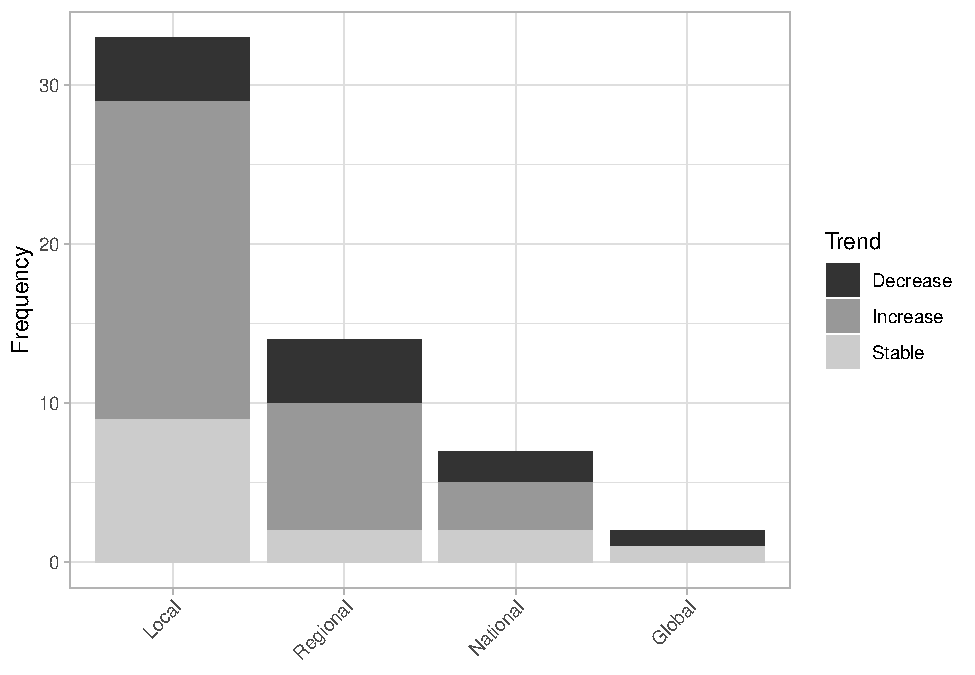
\includegraphics{literature_review_files/figure-latex/barspatscale-1.pdf}
\caption{\label{fig:barspatscale}Proportion of \emph{Increase}, \emph{Decrease} or \emph{Stable} trends for each spatial scale}
\end{figure}

\textbf{Trends by metric.} Among the different metrics, most of the examined studies deal with temporal trends of species richness and abundance (Figure \ref{fig:barmetrics}). The less common trend of abundance is \emph{Increase}, whilst \emph{Decrease} and \emph{Stability} are both as common. Diversity indexes (\emph{i.e.} Sørensen and Jaccard) were always found increasing and temporal \(\beta\)-diversity was found most of the time increasing and never decreasing. The use of the other metrics was rare.

\begin{figure}
\centering
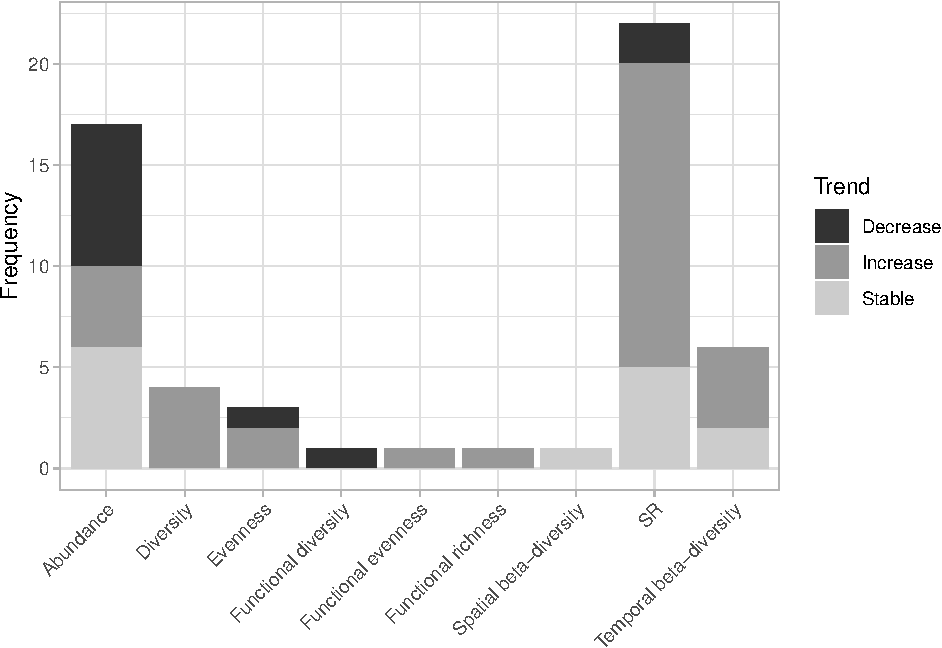
\includegraphics{literature_review_files/figure-latex/barmetrics-1.pdf}
\caption{\label{fig:barmetrics}Proportion of \emph{Increase}, \emph{Decrease} or \emph{Stable} trends for each of the metric}
\end{figure}

\textbf{Trends by spatial grain.} In the studies that we reviewed, at local grains, species richness mostly increased (Figure \ref{fig:barmetricsperspatscale}). Evenness indices, \emph{i.e.} taxonomic and functional evenness, were also mostly increasing. Concerning the abundance indices, we found mostly no trend, or increases. At regional grains, abundance metrics always decreased, temporal \(\beta\)-diversity always increased, and species richness increased. At national and global grains, studies analyzing multiple locations are rare, and most trends reported here for these two spatial scales are not replicated. Exceptions are \textcite{bowler_geographic_2021} and \textcite{donald_agricultural_2001}. The former showed negative trends in abundance indices for Denmark and Germany, and positive trends for Switzerland and Czech Republic, \emph{i.e.} no clear direction of the trend (here referred as \emph{Stable}). However, for \textcite{donald_agricultural_2001}, trends of mean population size were computed for 30 European countries and the majority was negative. Global trends only come from \textcite{jarzyna_taxonomic_2018}, who report a global decrease of species richness and a stable temporal \(\beta\)-diversity.

\begin{figure}
\centering
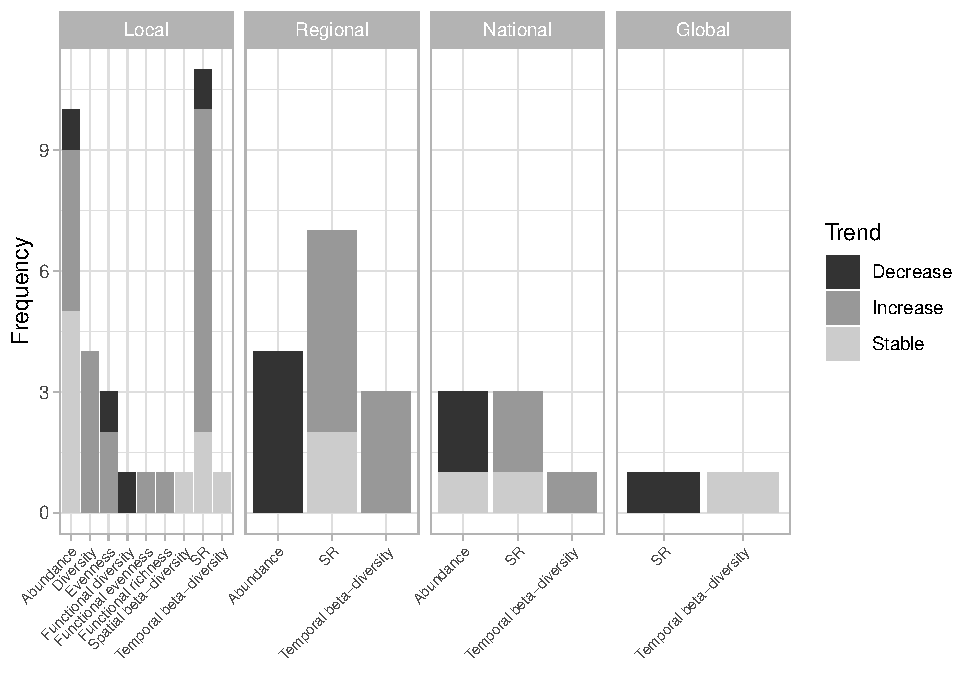
\includegraphics{literature_review_files/figure-latex/barmetricsperspatscale-1.pdf}
\caption{\label{fig:barmetricsperspatscale}Proportion of \emph{Increase}, \emph{Decrease} or \emph{Stable} trends for each metric. Each panel represent one spatial scale}
\end{figure}

However, concerning species richness, we can see that the decrease is global, but that this decrease is rare at finer spatial scales. In fact, we observe more often increases, confirming the high perturbations that biodiversity is undergoing \autocite{dornelas_assemblage_2014,vaidyanathan_worlds_2021}. This analysis goes along with the temporal \(\beta\)-diversity which is always observed either stable or increasing. Indeed, increasing turnover through time is a sign of an increasing perturbation of the ecosystems.

\hypertarget{temporal-scale-and-temporal-trends}{%
\chapter{Temporal scale and temporal trends}\label{temporal-scale-and-temporal-trends}}

The oldest study started in 1968 and the median duration is 23 years, with a minimum time-span of 11 years and a maximum of 45. We found longest temporal grains in studies with large spatial extent (Figure \ref{fig:spacetimegrain}). This is because data used in the selected article are mainly structured data, \emph{i.e.} data following a well established sampling plan. This type of survey is sparse since it needs resources and organization. Increasing the spatial extent thus increases both the temporal extent and the temporal grain. This explains this positive correlation between spatial extent and temporal grain. This limitation can be overcome thanks to citizen science data, which have increasingly been used \autocites[\emph{e.g.}][]{bowler_geographic_2021,isaac_data_2020,isaac_statistics_2014}. The opportunistic nature of these data allows for short census times, even over a large area. These data, with high temporal grain resolution for large spatial scales, could in future be used to explore in more details the temporal scaling of biodiversity trends.

Determination of the temporal grain in the studies in Table 1 was complicated. Usually, the temporal grain of the sampling was specified, but sometimes with inaccuracies (\emph{e.g.} \emph{``in the early morning''}). Moreover, the temporal grain of the sampling doesn't represent the temporal grain of the metric. For instance, some metrics are summed over a certain area \autocite[\emph{e.g.} summing the species richness over an atlas square, such as in][]{van_turnhout_scale-dependent_2007}. Analogically, the temporal grain should have also been summed over all the sampling censuses englobed in this area, but this was never the case. Moreover, when the trend is computed, usually the lag \autocite[\emph{i.e.} the time between two computation of the metric,][]{dungan_balanced_2002} is clearly specified, but the temporal grain is not.

For the cases where the metric of biodiversity is determined out of model \autocite[\emph{e.g.}][]{harrison_assessing_2014}, it is easier to assess the temporal grain, since predictions allow one to extrapolate the data from the sampling temporal grain to a wanted one. Thus, for these cases, the final temporal grain was most of the time explicitly given.

In short, temporal grain is rarely specified, especially when the metric computed makes it different from the sampling plan, or when the trend of the biodiversity metric is computed.

\begin{figure}
\centering
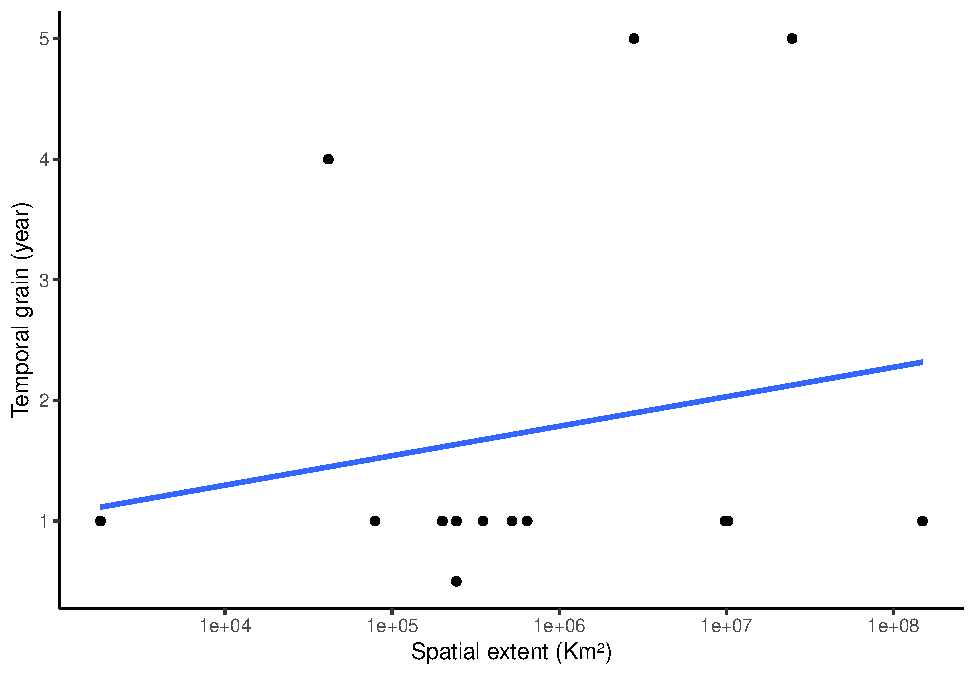
\includegraphics{literature_review_files/figure-latex/spacetimegrain-1.pdf}
\caption{\label{fig:spacetimegrain}Not sure about the relevance of this figure}
\end{figure}

\hypertarget{lack-of-spatial-replication}{%
\chapter{Lack of spatial replication}\label{lack-of-spatial-replication}}

Articles reporting trends from more than a single location are uncommon (we only found 17 of them), either due to a lack of data, or because the trend was assessed for the spatial extent of the data. For instance, the US Breeding Bird Survey \autocites[\emph{e.g.}][]{kamp_population_2021,sauer_north_2013} follows a standardized sampling plan with spatial replications (\emph{i.e.} multiple census plots). However, not all the trends reported for the BBS are summarized at their specific grain, and were sometimes aggregated over their respective national scales, reducing spatial replication. For instance, the common method encountered to assess population abundance trends (\emph{i.e.} abundance indexes) is to learn a predictive model from the data, predict the target feature (\emph{i.e.} abundance) and then compute the metric and its trend from the output of the model at the national spatial extent \autocites[\emph{e.g.}][]{doxa_low-intensity_2010,eglington_disentangling_2012,jiguet_french_2012,jiguet_modeling_2005,sauer_first_2017}. These analyses are practically useful for conservation, and are common \autocite{fraixedas_state_2020}: they give inform about ecosystem health at national extent, and are thus useful for decision-makers.

Another common type of study uses the \emph{space-for-time substitution} \autocite{walker_use_2010} to assess the trend of a metric \autocite[one of the best example is][]{hill_determining_2004}. This method consists in considering sampling in different places as representing a temporal trend. One could think that using theses studies could increase significantly the spatial replicates. However, the space-for-time substitution is mainly used to assess the impact of a processes (\emph{e.g.} before/after logging, before/after urbanization etc) meaning that the trend computed is highly biased, which we try to avoid for our topic.

Even fewer articles computed the trends of metrics with spatial replicates across more than one spatial grain. So far this was the case for only \textcite{chase_species_2019} and \textcite{jarzyna_taxonomic_2018}. Importantly, \textcite{jarzyna_spatial_2015} did spatial replicates of temporal change community metrics (\emph{i.e.} temporal dissimilarity, temporal turnover, extinction and colonization) at several spatial scales. However, the temporal trend of these metrics weren't considered and are therefore not reported in Table \ref{tab:maintable}.

\hypertarget{metric-heterogeneity}{%
\chapter{Metric heterogeneity}\label{metric-heterogeneity}}

In contrast to macroecology, applied ecology has offered multiparametric indices that aim to reflect multiple components of an ecosystem, the so-called \emph{composite indicators}. Examples are the red list index \autocite{butchart_improvements_2007} or biodiversity change indices \autocite{normander_indicator_2012}. The latter have proven effective for conservation policies. For birds, these indices have been widely used \autocite[see review by][]{fraixedas_state_2020}, while the use of simpler macroecological indices (\emph{e.g.} species richness, beta diversity) is uncommon.

\hypertarget{future-directions}{%
\chapter{Future directions}\label{future-directions}}

A striking but expected result \autocite[see][]{meyer_global_2015}, was the lack of studies form outside of the high-income global North. Out of 17 papers, 5 were located in North America and 12 in Europe. This is gap was also reported by \textcite{fraixedas_state_2020}. Yet, biodiversity dynamic in Europe may not be representative of global dynamic, and studies of biodiversity trends at several spatio-temporal scales are needed outside of Europe. These studies are needed on local grains, as well as at the spatial grain of continents \autocite[\emph{e.g.} as has been done by][ for amphibians and reptiles]{alroy_current_2015}.

The spatial grain of biodiversity trends is critical, yet this has not always been specified in the articles. One should consider the way a metric was computed, \emph{e.g.} if it was summed, modeled, averaged over the sampling units. According to the method, the spatial grain can vary from the sampling unit to the sampling extent. Given the importance of spatial scaling of biodiversity patterns \autocite{storch_untangling_2004}, one has to expect that it will be also important for its dynamic \autocite[\emph{e.g.}][]{chase_species_2019}. We thus argue that authors should pay extra attention to specifying the spatial grain for every metric of biodiversity trends.

The importance of temporal scaling of biodiversity is known since \textcite{grinnell_role_1922}, who used California birds to demonstrate the species-time relationship, which has since been proven to be common with other bird populations \autocite{white_two-phase_2004}. Thus, as spatial grain, temporal grain is known to be important to explicit. However, there is no consensus on the definition of temporal grain and is thus specified in various ways: sometimes very precised \autocite[\emph{e.g.} time of each census point, as in][]{schipper_contrasting_2016} and sometimes without explicit information \autocite[\emph{e.g.}][`The sites are visited twice a year (April to early May and late May to June), during which volunteers walk two parallel 1-km-long transect lines {[}\ldots{]}']{harrison_assessing_2014}. As for the spatial grain, the metric can vary according to the temporal grain and the way it is computed. However, when temporal trend of a metric is assessed, the temporal lag of the trend is often only specified (\emph{i.e.} time-span between \(t\) and \(t+1\)). In other words, when computing a trend, one usually uses a single point either every day, every month or every year. However, this temporal lag doesn't represent the temporal grain that interests us. If one wants to study the temporal scaling of biodiversity trends, a clear assessment of the temporal grain needs to be done systematically.

\hypertarget{conclusion}{%
\chapter{Conclusion}\label{conclusion}}

Reviewing the scientific literature on avian biodiversity trends give us a glimpse of what needs to be done to better understand the scaling of biodiversity dynamic. The first challenge is to find a common definition of spatial and temporal grain when computing the trend. We showed that these definitions vary according to the way the metric is computed. Whilst spatial grain of a trend is intuitively important for biodiversity, temporal grain is less often considered, especially when the temporal grain is computed. Finally, as birds are one of the most data-rich taxa of vertebrates, the challenges highlighted here will be even more severe for other groups.

\newpage
\begin{singlespacing}
\printbibliography[heading=bibintoc, title={References}]
\end{singlespacing}

\newpage

\hypertarget{supplementary-materials}{%
\chapter*{Supplementary materials}\label{supplementary-materials}}
\addcontentsline{toc}{chapter}{Supplementary materials}

\begin{landscape}\begingroup\fontsize{10}{12}\selectfont

\begin{longtable}[t]{>{\raggedright\arraybackslash}p{6.5em}>{\raggedright\arraybackslash}p{6.5em}>{\raggedright\arraybackslash}p{6.5em}>{\raggedright\arraybackslash}p{40em}}
\caption{\label{tab:notetable}Supplementary informations about each article}\\
\toprule
Reference & Spatial grain (Km²) & Trend & Note\\
\midrule
\endfirsthead
\caption[]{\label{tab:notetable}Supplementary informations about each article \textit{(continued)}}\\
\toprule
Reference & Spatial grain (Km²) & Trend & Note\\
\midrule
\endhead

\endfoot
\bottomrule
\endlastfoot
\cellcolor{gray!6}{\cite{barnagaud_temporal_2017}} & \cellcolor{gray!6}{Local} & \cellcolor{gray!6}{Increase} & \cellcolor{gray!6}{Not sure that it is at the road scale: "Taxonomic evenness showed a marginal, yet significant, non-linear increase from close to 0.54 in the first decade to 0.56 in the last decade (Table 1), suggesting a light trend towards a more even distribution of species’ abundances among species within local assemblages "}\\
 & Local & Increase & Mean change of SR at the road scales Area of the road = (40/0.8)*(pi*400\^2) with a road of 40 Km with point counts spaced by 0.8 Km and a census radius of 400m\\
\cellcolor{gray!6}{\cite{bowler_geographic_2021}} & \cellcolor{gray!6}{National} & \cellcolor{gray!6}{Stable} & \cellcolor{gray!6}{Metric = MSI, as many and as intense increase (i.e. Czech Rep. and Switzerland) than decrease (i.e. Germany and Denmarl)}\\
\cite{chase_species_2019} & Local & Stable & NA\\
\cellcolor{gray!6}{} & \cellcolor{gray!6}{Regional} & \cellcolor{gray!6}{Stable} & \cellcolor{gray!6}{\vphantom{1} NA}\\
\addlinespace
 & Regional & Stable & NA\\
\cellcolor{gray!6}{} & \cellcolor{gray!6}{Local} & \cellcolor{gray!6}{Increase} & \cellcolor{gray!6}{\vphantom{6} NA}\\
 & Local & Increase & \vphantom{5} NA\\
\cellcolor{gray!6}{\cite{chiron_forecasting_2013}} & \cellcolor{gray!6}{Regional} & \cellcolor{gray!6}{Decrease} & \cellcolor{gray!6}{Concerning the spatial scale, predictions are made using the spatial unit of 4 Km² and the FBI is computed for each region of France, then meanned. Prediction with baseline scenario}\\
 & Regional & Decrease & FBI prediction with CAP greening cenario\\
\addlinespace
\cellcolor{gray!6}{} & \cellcolor{gray!6}{Regional} & \cellcolor{gray!6}{Decrease} & \cellcolor{gray!6}{FBI prediction with No Pillar I scenario}\\
 & Regional & Decrease & FBI prediction with biofuel scenario\\
\cellcolor{gray!6}{\cite{davey_rise_2012}} & \cellcolor{gray!6}{Local} & \cellcolor{gray!6}{Increase} & \cellcolor{gray!6}{Metric = Simpson.They predict the metric using a GAM with spatial resolution of 1 Km². Then they show the trend for the mean value of the metric per year}\\
 & Local & Increase & \vphantom{4} NA\\
\cellcolor{gray!6}{} & \cellcolor{gray!6}{Local} & \cellcolor{gray!6}{Increase} & \cellcolor{gray!6}{\vphantom{3} NA}\\
\addlinespace
\cite{harrison_assessing_2014} & Local & Increase & To assess the metric, they use a GAM to predict the abundance over the entire area of interest (spatial resolution = 1 Km²) and then compute the geometric mean of species abundance = Multi Species Index (as in \cite{studeny_fine-tuning_2013}) from the prediction. Data used to learn the GAM are sampled from plots of 1 Km². Farmland communities\\
\cellcolor{gray!6}{} & \cellcolor{gray!6}{Local} & \cellcolor{gray!6}{Stable} & \cellcolor{gray!6}{Farmland communities, GoF ($\lambda$ = -1) =  weighted towards the rare species}\\
 & Local & Stable & Farmland communities, GoF ( $\lambda$ = -2) weighted towards the common species\\
\cellcolor{gray!6}{\cite{harrison_quantifying_2016}} & \cellcolor{gray!6}{Local} & \cellcolor{gray!6}{Increase} & \cellcolor{gray!6}{Geomteric mean of species abundance, they predict the abundance with resolution of 1 Km² and then computed the metric for each 10000 Km² cell across Great Britain, Visited twice a year}\\
 & Local & Stable & GoF ( $\lambda$ = -1) = toward rare species" The goodness-of-fit-based measure of biodiversity suggests that both rare and common species made gains through much of Britain in the first half of the time period, and losses in the second half.", Visited twice a year / Increase first half and second second halfGoF ( $\lambda$ = -1)\\
\addlinespace
\cellcolor{gray!6}{} & \cellcolor{gray!6}{Local} & \cellcolor{gray!6}{Stable} & \cellcolor{gray!6}{GoF ( $\lambda$ = -2) = toward common species " The goodness-of-fit-based measure of biodiversity suggests that both rare and common species made gains through much of Britain in the first half of the time period, and losses in the second half.", Visited twice a year / Increase first half and second second half}\\
\cite{jarzyna_taxonomic_2018}\cellcolor{gray!6}{} & \cellcolor{gray!6}{Regional} & \cellcolor{gray!6}{Increase} & \cellcolor{gray!6}{\vphantom{4} NA}\\
 & Regional & Increase & \vphantom{3} NA\\
\cellcolor{gray!6}{} & \cellcolor{gray!6}{Regional} & \cellcolor{gray!6}{Increase} & \cellcolor{gray!6}{\vphantom{2} NA}\\
\cellcolor{gray!6}{} & \cellcolor{gray!6}{National} & \cellcolor{gray!6}{Increase} & \cellcolor{gray!6}{\vphantom{1} NA}\\
\addlinespace
 & Global & Decrease & NA\\
 & Regional & Increase & \vphantom{1} NA\\
\cellcolor{gray!6}{} & \cellcolor{gray!6}{Regional} & \cellcolor{gray!6}{Increase} & \cellcolor{gray!6}{NA}\\
 & Regional & Increase & NA\\
 & National & Increase & NA\\
\addlinespace
\cellcolor{gray!6}{} & \cellcolor{gray!6}{Global} & \cellcolor{gray!6}{Stable} & \cellcolor{gray!6}{NA}\\
\cite{pilotto_meta-analysis_2020}\cellcolor{gray!6}{} & \cellcolor{gray!6}{Local} & \cellcolor{gray!6}{Stable} & \cellcolor{gray!6}{"Analyses of the trends in local biodiversity over large spatial scales"}\\
\cellcolor{gray!6}{} & \cellcolor{gray!6}{Local} & \cellcolor{gray!6}{Increase} & \cellcolor{gray!6}{Metric = Simpson, "Analyses of the trends in local biodiversity over large spatial scales"}\\
 & Local & Increase & "Analyses of the trends in local biodiversity over large spatial scales"\\
 & Local & Stable & "Analyses of the trends in local biodiversity over large spatial scales"\\
\addlinespace
\cite{ram_what_2017} & Local & Increase & MSI for forest species, road of 8 Km with no limitations so assumed 200m\\
\cellcolor{gray!6}{} & \cellcolor{gray!6}{Regional} & \cellcolor{gray!6}{Increase} & \cellcolor{gray!6}{SR for forest species meaned over roads, spatial grain = 8* .4 with road of 8 Km and census radius no limitations so assumed 200m}\\
\cite{reif_changes_2013} & Local & Stable & Jaccard index, pairwise comparisions between transects\\
\cellcolor{gray!6}{} & \cellcolor{gray!6}{Local} & \cellcolor{gray!6}{Stable} & \cellcolor{gray!6}{JPSP data, transect scale}\\
 & National & Stable & JPSP data, national scale\\
\addlinespace
\cellcolor{gray!6}{\cite{schipper_contrasting_2016}} & \cellcolor{gray!6}{Local} & \cellcolor{gray!6}{Increase} & \cellcolor{gray!6}{The metric (i.e. geometric mean) is meaned over each road. Area of the road = 50*(pi*400\^2) with 50 census point per road and a census radius of 400m}\\
 & Local & Increase & Metric = Shannon\\
\cellcolor{gray!6}{} & \cellcolor{gray!6}{Local} & \cellcolor{gray!6}{Increase} & \cellcolor{gray!6}{Metric = Simpson}\\
 & Local & Decrease & NA\\
\cellcolor{gray!6}{} & \cellcolor{gray!6}{Local} & \cellcolor{gray!6}{Increase} & \cellcolor{gray!6}{\vphantom{2} NA}\\
\addlinespace
 & Local & Increase & \vphantom{1} NA\\
\cellcolor{gray!6}{} & \cellcolor{gray!6}{Local} & \cellcolor{gray!6}{Increase} & \cellcolor{gray!6}{NA}\\
\cite{sorte_changes_2005} & Local & Decrease & NA\\
\cellcolor{gray!6}{} & \cellcolor{gray!6}{Local} & \cellcolor{gray!6}{Decrease} & \cellcolor{gray!6}{Metric = evenness}\\
 & Local & Increase & The metric is meaned over each road. Area of the road = 50*(pi*400\^2) with 50 census point per road and a census radius of 400m\\
\addlinespace
\cellcolor{gray!6}{\cite{van_turnhout_scale-dependent_2007}} & \cellcolor{gray!6}{Regional} & \cellcolor{gray!6}{Increase} & \cellcolor{gray!6}{For each region, the trend is computed using the mean number of species per atlas square}\\
 & Local & Increase & Mainly increase of SR but the proportion of negative trend were higher than for the regional scale\\
\cellcolor{gray!6}{} & \cellcolor{gray!6}{National} & \cellcolor{gray!6}{Increase} & \cellcolor{gray!6}{National scale}\\
\cite{wretenberg_changes_2010} & Local & Decrease & looking at the trend through different environmental policies, " local species richness (i.e. at the scale of sites = 3 hectares) decreased significantly probably as a result of an overall reduced abundance of several species. "\\
\cellcolor{gray!6}{\cite{inger_common_2015}} & \cellcolor{gray!6}{National} & \cellcolor{gray!6}{Decrease} & \cellcolor{gray!6}{NA}\\
\addlinespace
\cite{donald_agricultural_2001} & National & Decrease & The metric is referred as "Mean population" and the trend is estimated for each european country\\*
\end{longtable}
\endgroup{}
\end{landscape}


%%%%%%%%%%%%%%%% Here is the part that I am using for the bibliography to be displayed in the toc
%%% First step: I define the name and label of the biblio part
%%\chapter{References}\label{references}
%%{
%%% I temporarily redefine the clearpage in order for the bib to not be printed on a new page
%%\renewcommand{\clearpage}{}
%%\printbibliography[heading=none] % I delete the default name of the bib
%%\printbibliography 
%%}
%
\end{document}
